\newpage
\section{Revisão da Teoria}

\subsection{OFDM}

Matematicamente, uma única portadora (figura \ref{fig:spec-a}) pode ser descrita pela seguinte equação:

\begin{equation}
s_c(t) = A_c(t)b_ce^{j|\omega_c t + \phi_c (t)|},
\end{equation}

sendo $A_c$ a amplitude, $b_c$ é o vetor de dados, $\omega_c$ e  $\phi_c (t)$ a frequência angular e a fase do sinal modulado, respectivamente \cite{Alencar}.

O sinal OFDM consiste de várias portadoras, conforme mostra a figura \ref{fig:spec-b}, que são descritas pela equação 

\begin{equation}
s_{ofdm} = \frac{1}{N} \sum_{n=0}^{N-1}A_n(t)e^{j|\omega_n t + \phi_n (t)|},
\end{equation}

onde N é o número de portadoras, ou canais e $\omega_n = \omega_c + n\Delta\omega$.

\begin{figure}[H]
  \centering
  \caption{Espectro do sinal OFDM.}
  
  \subfloat[Uma portadora]{\label{fig:spec-a}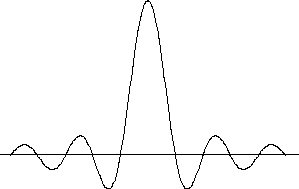
\includegraphics[scale=0.6]{spectrum-a}}\\
  
  \subfloat[Cinco portadoras]{\label{fig:spec-b}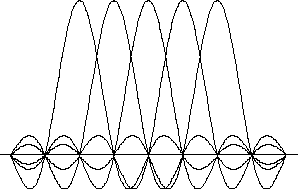
\includegraphics[scale=0.6]{spectrum-b}}
  
  \small Fonte: Matic, D., \textit{Mathematical description of OFDM} (2015).
\end{figure}

É importante notar que todas as portadoras devem, obrigatoriamente, ser ortogonais, para que não haja interferência na transmissão.

\begin{figure}[H]
  \centering
  \caption{Estrutura de um sistema de transmissão multicanal.}
  \label{fig:tx}
  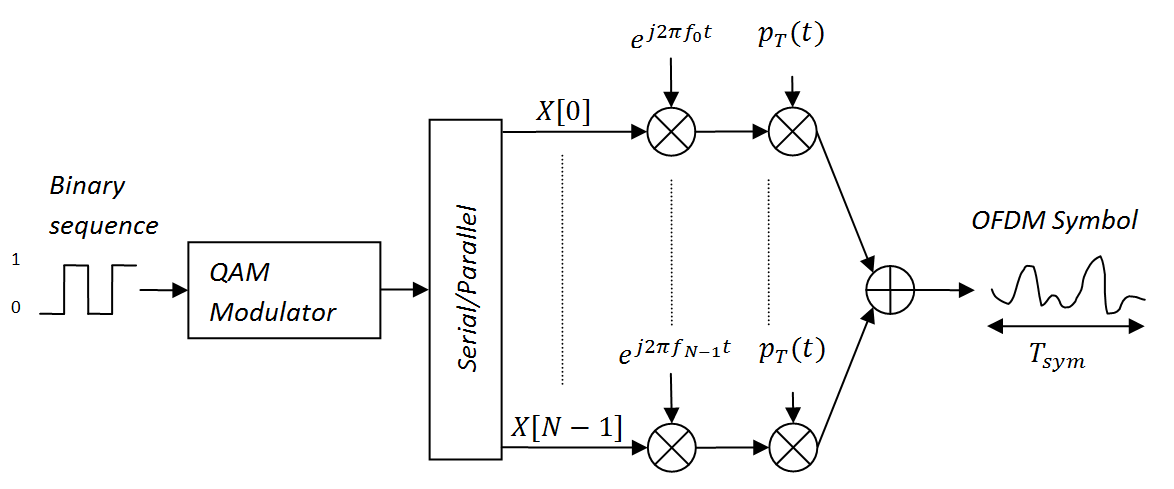
\includegraphics[scale=0.4]{mod}
  
  \small Fonte: Fonte: Matic, D., \textit{Mathematical description of OFDM} (2015).
\end{figure}

A figura \ref{fig:tx} mostra a estrutura básica de um transmissor OFDM com modulação QAM, onde é possível notar a separação dos dados de entrada, que chegam de forma serial, em N subportadoras, igualmente espaçadas por $\Delta N$, sendo

\begin{equation}
\Delta f = \frac{\Delta \omega}{2 \pi} = \frac{1}{NT}.
\end{equation}

\subsection{Sistemas OFDM com transformada de Fourier}
A principal razão pela qual os sistemas OFDM demoraram a aparecer em produtos de uso civil é a dificuldade de gerar os sinais e, ainda mais difícil, receber e demodular o sinal recebido. A solução via hardware, com múltiplos moduladores e demoduladores, tornava inviável o uso da técnica, devido a grande complexidade e alto custo de implementação.

Com o avanço da tecnologia nos DSPs e FPGAs, foi possível utilizar a transformada inversa de Fourier para gerar os sinais OFDM, reduzindo drasticamente o custo de tais sistemas. De forma complementar, na recepção e demodulação, pode ser utilizada a transformada discreta de Fourier, simplificando os sistemas OFDM.

\begin{figure}[H]
  \centering
  \caption{Estrutura de um sistema OFDM com transformada de Fourier.}
  \label{fig:fourier}
  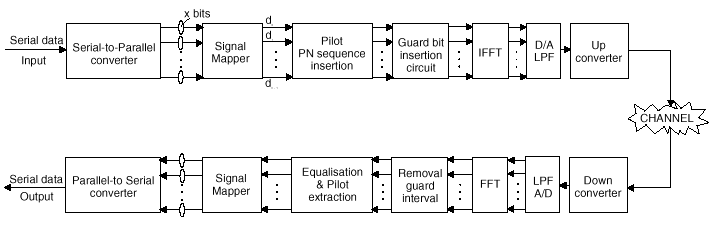
\includegraphics[width=\textwidth]{fourier}
  
  \small Fonte: Fonte: Matic, D., \textit{Mathematical description of OFDM} (2015).
\end{figure}

No transmissor, o sinal é definido no domínio da frequência. Ele é amostrado de modo digital e é definido de tal maneira que o espectro discreto de Fourier exista somente em frequências discretas. Cada portadora do sistema OFDM corresponde a um elemento desse espectro discreto. Dessa forma, a amplitude e fase das portadoras dependem do dado a ser transmitido. As transições dos dados são sincronizadas nas portadoras, podendo ser processadas em conjunto, símbolo por símbolo.

A figura \ref{fig:fourier} mostra um esquema OFDM com o uso da transformada de Fourier.

